\section{Setup}

Our evaluation cluster comprises two Intel(R) Xeon(R) Gold systems, 
each with 48 cores and 48 hyperthreads running at 2.40GHz. The systems 
are equipped with 260 GB RAM, 72 MB aggregate cache, and an Intel E810 
100Gb Ethernet adapter. One of the systems serves as the server, while 
the other is used for clients. All the machines run Debian GNU/Linux 11 
(bullseye) with kernel version 5.15, and we use Open vSwitch version 3.1.0. 
We build TAS using DPDK 21.11.

\section{Single flow overhead}

\textbf{Throughput}

\begin{figure}
    \centering
    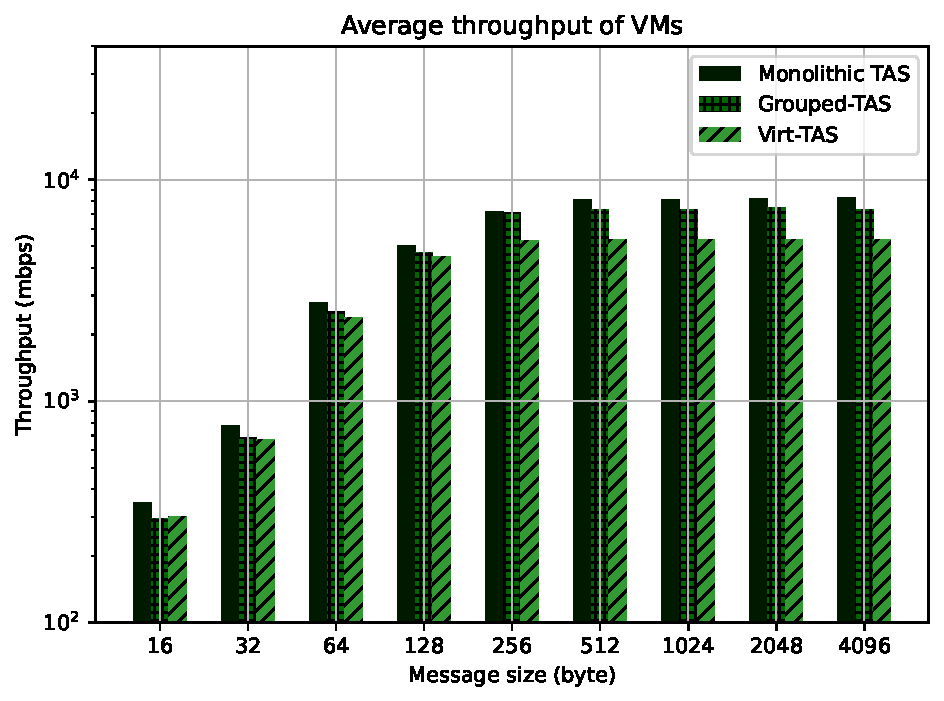
\includegraphics[scale=0.8]{../results/overhead.throughput.pdf}
    \caption{Single context overhead.}
    \label{fig:overhead.throughput}
\end{figure}

\textbf{Latency}





\section{Multiplexing}

The goal of multiplexing experiment is to validate the enhancement of VirtTAS in terms of 
higher throughput and resource efficiency. Specifically, the experiment 
investigates the ability of VirtTAS to benefit from multiplexing of packet processing 
across multiple VMs through a shared TCP fast-path. 

To this end, we conduct three different scenarios, as illustrated in Figure 
\ref{fig:multiplexing.experiment}. In each of the scenarios, we configure four 
VMs across two servers. The servers in this experiment are interconnected directly. 
Subsequently, we execute Micro-RPC benchmarks between four pairs of VMs, 
with message sizes from 16 to 4096.


In the first scenario (\emph{kernel}), we follow the conventional 
setup where applications running on the VMs utilize the conventional kernel 
networking. In this scenario, the hypervisor establishes connectivity to VMs through 
TAP devices, while a virtual switch applies virtualization policies to the network. 
For the setup, we allocate three cores to each VM. The server and client applications 
are using three threads to leverage all available cores. 
Additionally, the virtual switch runs on a separate core. Overall, the scenario employs
a total of 13 cores. 

In the second scenario (\emph{Independent-TAS}), we execute the TCP acceleration service on each VM, 
utilizing two cores for the service and one core for the application itself. 
The goal is to optimize TCP packet processing within the VMs, 
to increase throughput and reduce latency for the applications. 
Similar to the first scenario, the virtual switch applies virtualization policies 
to packets on the hypervisor, and the experiment consumes 13 cores.


In the final scenario (\emph{Virt-TAS}), we deployed VirtTAS on the hypervisor, dedicating four 
cores exclusively to its operations. In this case, each VM is allocated a single 
core for application processing. Notably, this scenario requires only 8 cores,
which is nearly 40\% less cores comparing to previous scenarios.


Figure \ref{fig:multiplex.throughput} illustrates the average throughput of 
Micro-RPC benchmark in three aforementioned different scenarios. 
The analysis indicates that, for message sizes smaller than 256, VirtTAS outperforms 
the alternative methods. Specifically, for message of size 256, VirtTAS yields
a 25\% higher average throughput than the kernel case, and for message size 64, 
VirtTAS achieves \(2\times\) the throughput of the kernel case.

Based on the results presented in Figure \ref{fig:multiplex.throughput}, it is 
evident that in scenarios where the cloud provider does not offer the TCP Acceleration 
Service (TAS), they can still take advantage of fast-path TCP by deploying TAS on their 
VMs for workloads with message sizes of less than 32 bytes.

\begin{figure}
    \centering
    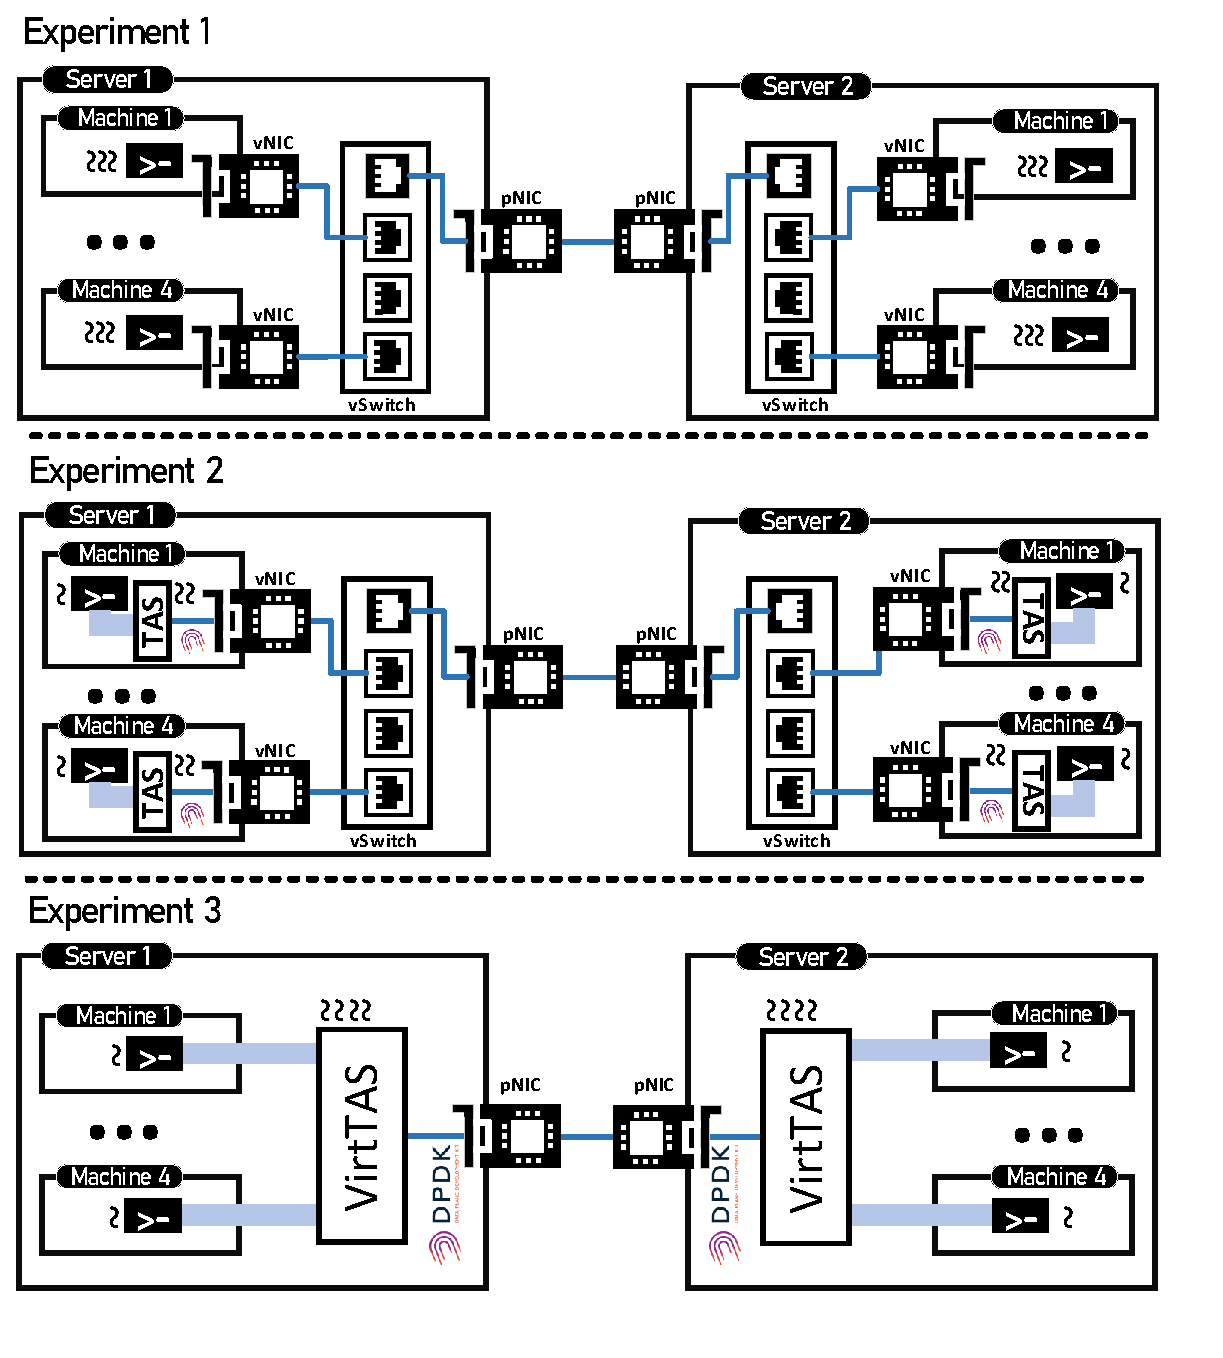
\includegraphics[scale=0.6]{../Figures/multiplexing.experiment.pdf}
    \caption{Multiplexing experiment setup in three different scenarios (\emph{i}) kernel, 
    (\emph{ii}) Independent-TAS, and (\emph{iii}) Virt-TAS.}
    \label{fig:multiplexing.experiment}
\end{figure}

\begin{figure}
    \centering
    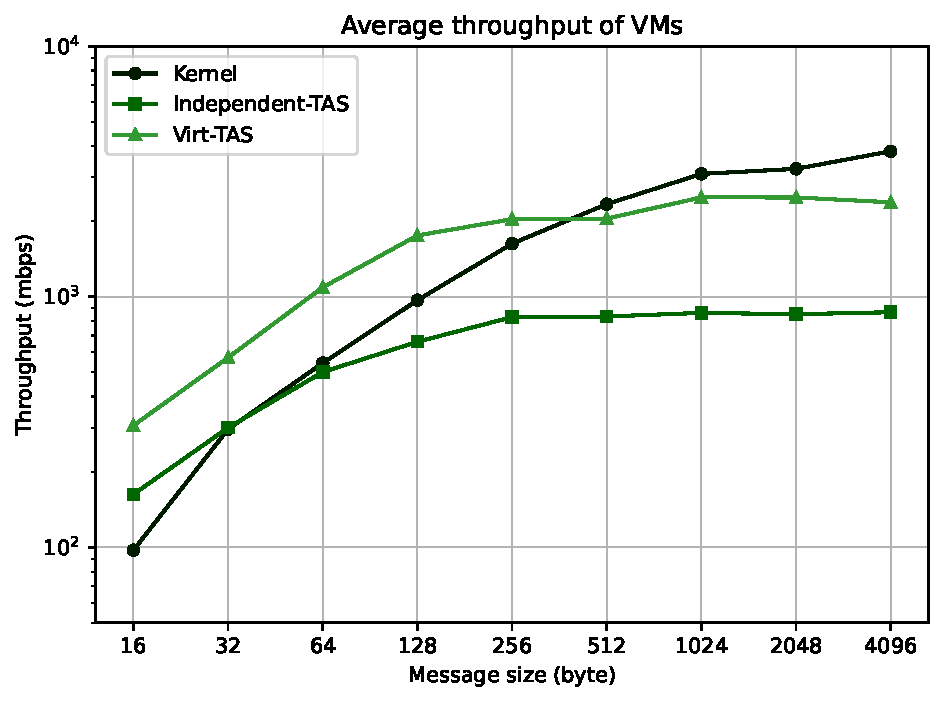
\includegraphics[scale=0.6]{../results/multiplex.throughput.pdf}
    \caption{Average throughput of Micro-RPC benchmark in three different scenarios (\emph{i}) kernel, 
    (\emph{ii}) Independent-TAS, and (\emph{iii}) Virt-TAS}
    \label{fig:multiplex.throughput}
\end{figure}
